% These are the lecture notes for my CSCI360 course SPRING 2017
% at John Jay College of Criminal Justice.

% Feel free to edit these slides and use them for your own courses.
% HOWEVER DO NOT REMOVE THESE LINES!
% Email me at: awood [at] jjay.cuny.edu
% or at: awood [at] gradcenter.cuny.edu


\documentclass{beamer}

\usepackage{tikz}
\usetikzlibrary{calc}

\usepackage{forest}
\usepackage{verbatim}
\usepackage{color}


\setbeamertemplate{footline}[frame number]
\setbeamertemplate{navigation symbols}{} 

\newtheorem{thm}{Theorem}[section]
\newtheorem{lem}{Lemma}
\newtheorem{cl}{Claim}
\newtheorem{cor}{Corollary}[section]
\newtheorem{conj}{Conjecture}
\newtheorem{quest}{Question}
\newtheorem{defn}{Definition}[section]
\newtheorem{obs}{Observation}[section]
\newtheorem{exam}{Example}

\newcommand{\im}{\operatorname{im}}
\newcommand{\id}{\operatorname{id}}
\newcommand{\interior}{\operatorname{int}}
\newcommand{\bdry}{\operatorname{bdry}}
\newcommand{\<}{\langle}
\renewcommand{\>}{\rangle}
\newcommand{\Gab}{(G_\phi)^{ab}} 
\newcommand{\phibar}{\bar{\phi}}
\newcommand{\Z}{\mathbb{Z}}
\newcommand{\N}{\mathbb{N}}
\newcommand{\Q}{\mathbb{Q}}
\newcommand{\R}{\mathbb{R}}
\newcommand{\C}{\mathbb{C}}
\newcommand{\A}{\mathcal{A}}
\newcommand{\OO}{\mathcal{O}}
\newcommand{\UU}{\mathcal{U}}
\newcommand{\power}{2^{\{P_1, \cdots , P_n\}}}
\newcommand{\bp}{\begin{problem}}
\newcommand{\ep}{\end{problem}}
\newcommand{\ba}{\begin{answer}}
\newcommand{\ea}{\end{answer}}
\newcommand{\ds}{\displaystyle}
\newcommand{\ben}{\renewcommand{\theenumi}{\alph{enumi}}
\renewcommand{\labelenumi}{(\theenumi)}\begin{enumerate}}
\newcommand{\een}{\end{enumerate}}
\newcommand{\Hess}{\operatorname{Hessian}}
\newcommand{\Aut}{\mathrm{Aut}}
\newcommand{\Inn}{\mathrm{Inn}}
\newcommand{\Out}{\mathrm{Out}}
\newcommand{\End}{\mathrm{End}}


\mode<presentation>
{
%  \usetheme{default}
  \setbeamercovered{invisible}
}


\usepackage[english]{babel}
\usepackage[latin1]{inputenc}
\usepackage{times}
\usepackage[T1]{fontenc}
\usepackage{stmaryrd}

%\usetheme{default}
%\usetheme{AnnArbor}
%\usetheme{Antibes}
%\usetheme{Bergen}
%\usetheme{Berkeley}
%\usetheme{Berlin}
%\usetheme{Boadilla}
%\usetheme{CambridgeUS}
%\usetheme{Copenhagen}
%\usetheme{Darmstadt}
%\usetheme{Dresden}
%\usetheme{Frankfurt}
%\usetheme{Goettingen}
%\usetheme{Hannover}
%\usetheme{Ilmenau}
%\usetheme{JuanLesPins}
%\usetheme{Luebeck}
%\usetheme{Madrid}
%\usetheme{Malmoe}
%\usetheme{Marburg}
%\usetheme{Montpellier}
%\usetheme{PaloAlto}
%\usetheme{Pittsburgh}
%\usetheme{Rochester}
\usetheme{Singapore}
%\usetheme{Szeged}
%\usetheme{Warsaw}

%\usecolortheme{default}
%\usecolortheme{albatross}
\usecolortheme{beaver}
%\usecolortheme{beetle}
%\usecolortheme{crane}
%\usecolortheme{dolphin}
%\usecolortheme{dove} % grey, white, yellow
%\usecolortheme{fly} %grey, yellow
%\usecolortheme{lily} %white, yellow, blue
%\usecolortheme{orchid}
%\usecolortheme{rose}
%\usecolortheme{seagull}
%\usecolortheme{seahorse}
%\usecolortheme{whale}
%\usecolortheme{wolverine}

% Title page

\title[CSCI360]{Coding Vigen\`{e}re's Cipher Using Python \\ (Based off of \emph{Invent With Python} Chapter 19)}

\author
{Lecture notes of Alexander Wood \\ CSCI 360 Cryptography and Cryptanalysis \\ \scriptsize \href{mailto:awood@jjay.cuny.edu}{awood@jjay.cuny.edu}}
\institute[JJay]{John Jay College of Criminal Justice}  

\date{}

\begin{document}

% Remove 'figure' text from figure captions 
\setbeamertemplate{caption}{\raggedright\insertcaption\par}

\begin{frame}
  \titlepage
\end{frame}

\begin{frame}
These slides are based off of Chapter 19 of \emph{Invent With Python}, available at the link below:
\begin{center}
\url{https://inventwithpython.com/hacking/chapter19.html}
\end{center}
All images and information are taken from this page unless otherwise noted.
\end{frame}


\begin{frame}
\frametitle{Vigen\`{e}re's Cipher}

Today we will write code for Vigen\`{e}re's Cipher, described in the previous lecture.
\end{frame}


\begin{frame}
\frametitle{History: Discovery}
\begin{columns}
\begin{column}{0.5\textwidth}
\begin{figure}
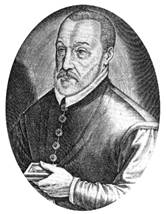
\includegraphics[scale=1]{IMG/vigenere.jpg}
\caption{Vigenere (1523 - 1596)}
\end{figure}
\end{column}

\begin{column}{0.5\textwidth}
The first record of this cipher is from 1553, penned by Italian cryptographer Giovan Battista Bellaso. It was later reinvented and popularised by Blaise de Vigen\`{e}re.
\end{column}
\end{columns}
\end{frame}


\begin{frame}
\frametitle{History: Breaking Vigenere}
\begin{columns}
\begin{column}{0.5\textwidth}
\begin{figure}
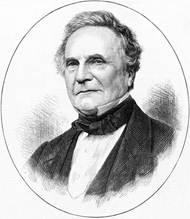
\includegraphics[scale=1]{IMG/babbage.jpg}
\caption{Babbage (1791-1871)}
\end{figure}
\end{column}

\begin{column}{0.5\textwidth}
This cipher remained unbroken until the 19th century! 
For a long time it was known as ``le chiffre ind\'{e}chiffrable'' (``the indecipherable cipher'').\newline

Charles Babbage (the ``father of computers'') was the first person known to break this cipher. 
\end{column}
\end{columns}
\end{frame}


\begin{frame}
\frametitle{Vigen\`{e}re's Cipher}

First, Alice (A) and Bob (B) decide upon a keyword. This is done offline, privately. Encryption follows the following steps:
\begin{enumerate}[1)]
\item Write out the plaintext message
\item Below it, write out the keyword, aligning each letter of the keyword below each letter of the plaintext. Repeat the keyword over and over until you reach the end of the plaintext. 
\item ``Add" these letters together using their values modulo 26, as computed in the coding exercises in the previous slides. (\emph{Note that this corresponds to a different Caeser shift for each letter in the keyword!})
\end{enumerate}
\end{frame}

\begin{frame}
\frametitle{A Helpful Chart}

For hand computations we can use the chart provided at \url{http://www.counton.org/explorer/codebreaking/vigenere-cipher.php}. 
\begin{figure}
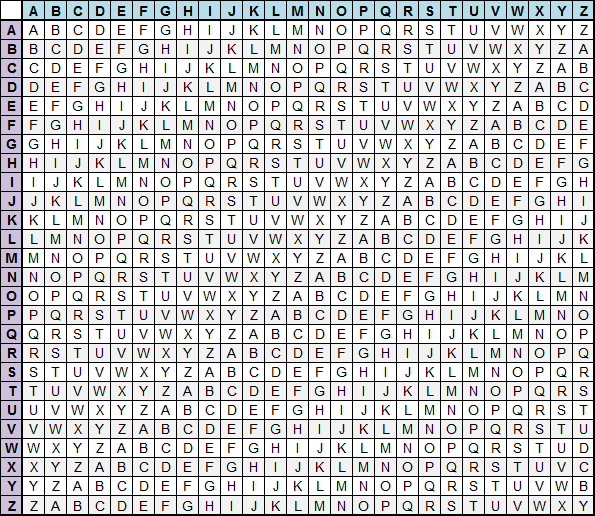
\includegraphics[scale=.4]{IMG/vignere.png}
\end{figure}
\end{frame}



\begin{frame}[fragile]
\frametitle{Vigen\`{e}re's Cipher: Multiple Caesar Shifts}

The key in Vigen\`{e}re is a sequence of letters. Each letter can be considered a subkey. For instance, below the keyword is \verb|PIZZA|. This image illustrates the use of the Caeser shift wheel for each letter in the key. 

\begin{figure}
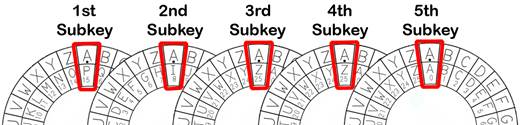
\includegraphics[scale=.8]{IMG/caesar.jpg}
\end{figure}
\end{frame}


\begin{frame}
\frametitle{I got the keys}

Last class we discussed how there are too many keys in Vigen\`{e}re's Cipher for a brute force attack to be successful.
\begin{figure}
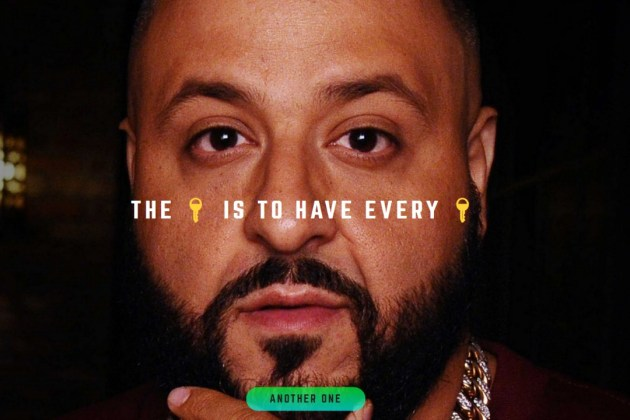
\includegraphics[scale=.3]{IMG/keys.jpg}
\end{figure}
How can we determine the keyspace of Vigen\`{e}re?
\end{frame}


\begin{frame}
\frametitle{Keyspace}

The size of the keyspace is determined by the length of the keyword!

\begin{figure}
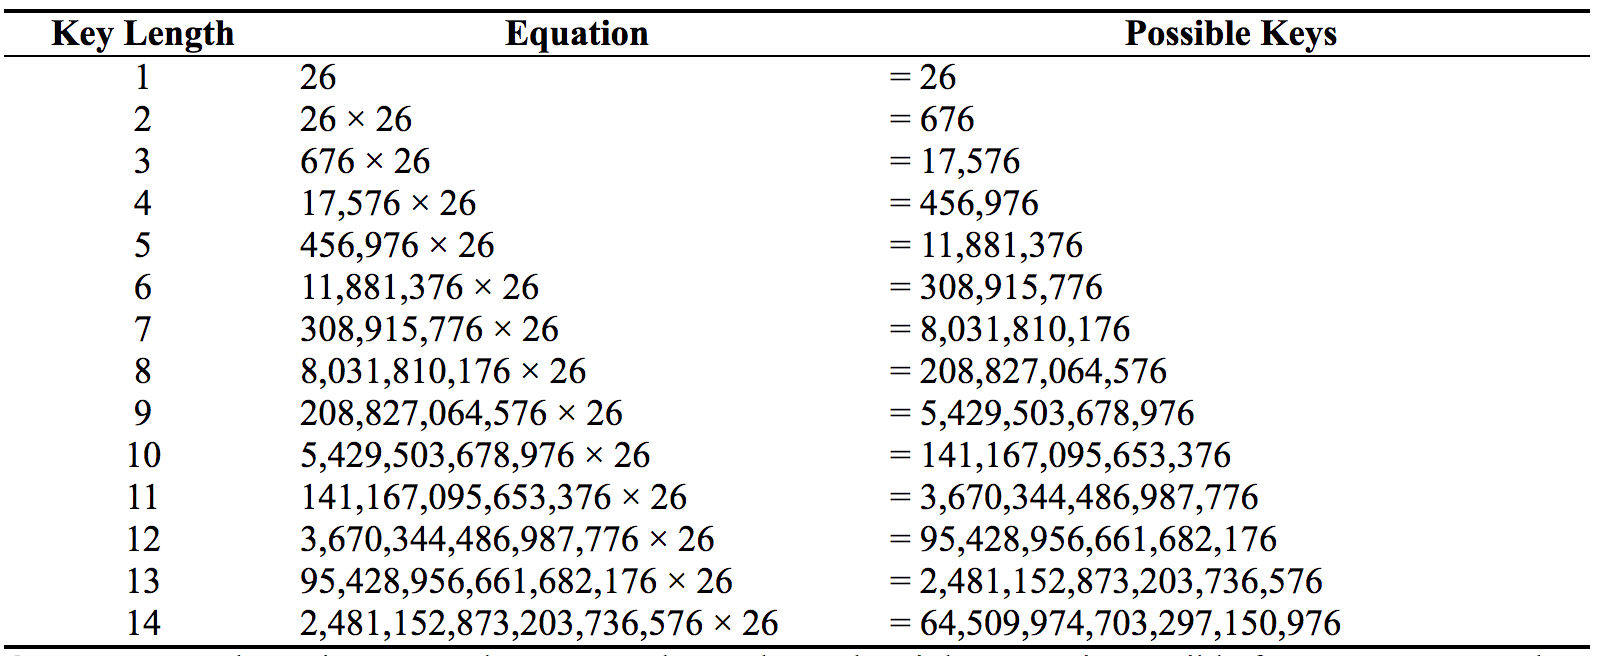
\includegraphics[scale=.4]{IMG/keyspace.png}
\end{figure}
\end{frame}


\begin{frame}[fragile]
\frametitle{Coding Vigen\`{e}re}

Now let's code Vigen\`{e}re's cipher. The code will consist of three functions:
\begin{itemize}
\item \verb|keygen|, which generates the key;
\item \verb|encrypt|, and
\item\verb|decrypt|
\end{itemize}
\end{frame}


\begin{frame}[fragile]
\frametitle{Coding: Keygen}

The \verb|keygen| function is somewhat trivial in this case; simply ask the user what key they would like to use and return this value. \newline

What sort of error-checking can we include to make sure that the key is correctly constructed? (No lower-case letters, no spaces, no punctuation, etc)?
\end{frame}


\begin{frame}[fragile]
\frametitle{Coding: Encrypt}

Make sure that you strip all spaces out of the plaintext message and make sure the plaintext is capitalized.

\end{frame}

\begin{frame}
\frametitle{Coding: Decrypt}

Now let's write the decryption function. If get the ciphertext by adding the plaintext to the keyword, how do we get the plaintext from the ciphertext?\newline

\emph{Answer: We get the plaintext by subtracting the keyword from the ciphertext.}
\end{frame}

\begin{frame}
\frametitle{References}

These slides are based off of Chapter 19 of \emph{Invent With Python}, available at the link below:
\begin{center}
\url{https://inventwithpython.com/hacking/chapter19.html}
\end{center}
\end{frame}
\end{document}


